\documentclass{article}
\usepackage{graphicx}
\usepackage{cite}
\usepackage{tikz}
\usepackage{amsmath}
\usepackage{mathtools}
\usepackage{bm}
\usetikzlibrary{patterns}
\usetikzlibrary{fit}
\usetikzlibrary{calc}
\usetikzlibrary{matrix}
\usetikzlibrary{positioning}
\usetikzlibrary{shapes.arrows}
\usepackage{makecell}
\usepackage{pgfplots}
\usepgfplotslibrary{groupplots,dateplot}
\pgfrealjobname{figures}
\pgfplotsset{compat=newest}
\usepackage{rotating}
\usepackage{amssymb}
\usepackage[english]{babel}

\DeclareUnicodeCharacter{2212}{−}




\begin{document}

	\beginpgfgraphicnamed{figures-observations}
	\begin{tikzpicture}

	% Crossing
	
	\draw[thick] (-5, 1) -- (-1, 1) -- (-1, 5);
	\draw[thick] (-5, -1) -- (-1, -1) -- (-1, -2);
	\draw[thick] (1, 5) -- (1, 1) -- (2, 1);
	\draw[thick] (1, -2) -- (1, -1) -- (2, -1);
	
	\draw (-3, 0) -- (2, 0);
	\draw (0, 3) -- (0, -2);
	
	% cars
	\node[inner sep=0pt] (ego_car) at (-4,0)
	{
\includegraphics[width=.18\textwidth, angle=0]{ego_car_top_down.png}};
%		\draw (-5, -0.5) rectangle ++(2, 1);
	\node[inner sep=0pt] (ego_car) at (0,4)
	{
\includegraphics[width=.18\textwidth, angle=-90]{target_car_top_down.png}};
%		\draw (-0.5, 3) rectangle ++(1, 2);
	
	\draw[->] (-3, 0.3) -- node[above] {$v^{ego}$} (-2, 0.3);
	\def\x{0.2}
	\draw[->] (\x, 3) -- (\x, 1.5);

	\draw (\x, 2.8) node[right] {$v^{j}$} (\x, 2.5) 
		-- node[right] {$i^{j}_\mathrm{take}$} (\x, 2) 
		-- node[right] {$i^{j}_\mathrm{give}$} (\x, 1.5);
%		\draw[->] (-3, -0.3) -- node[below] {$a_{ego}$} (-2, -0.3);
	
	% Disatance
	\draw (0,0) circle (5pt);
	% \node at (1.2, -0.3) {crossing point};
	
	% \def\x{-1}
	% \def\y{-2}
	% \draw (\x, \y) -- node[below] {$\delta^e$} (0, \y); 
	% \draw (\x, \y+0.1) -- (\x, \y-0.1);
	\def\x{-3}
	\def\xend{-1}
	\def\y{-0.4}
	\draw (\x, \y) -- node[below] {$p_\mathrm{int}^\mathrm{ego}$} (\xend, \y);
	\draw (\x, \y+0.1) -- (\x, \y-0.1);
	\draw (\xend, \y+0.1) -- (\xend, \y-0.1);
	
	\def\x{-3}
	\def\xend{1.5}
	\def\y{-1.4}
	\draw (\x, \y) -- node[below] {$p_\mathrm{goal}^\mathrm{ego}$} (-1, \y) -- (\xend, \y);
	% \draw (-1, \y)-- (\xend, \y);
	\draw (\x, \y+0.1) -- (\x, \y-0.1);
	\draw (\xend, \y+0.1) -- (\xend, \y-0.1);

	\def\x{-0.2}
	\def\y{3}
	\def\yend{1}
	\draw (\x, \y) -- node[left] {$p^{j}_\mathrm{int}$} (\x, \yend);
	\draw (\x-0.1, \y) -- (\x+0.1, \y);
	\draw (\x-0.1, \yend) -- (\x+0.1, \yend);
%	\def\x{2}
%	\def\y{0}
%	\draw (\x, \y) -- node[right] {$\delta^j$} (\x, 1);
%	\draw (\x-0.1, \y) -- (\x+0.1, \y);
	
	\end{tikzpicture}\\
	\endpgfgraphicnamed

	\beginpgfgraphicnamed{figures-conflict_car}
	\begin{tikzpicture}

	% Crossing
	\def\crossverticalx{0}
	\def\crosstopy{8}
	\def\crossboty{-2.5}
	\def\crossleftx{-7}
	
	\draw[thick] (\crossleftx, 1) -- (-1, 1) -- (-1, \crosstopy);
	\draw[thick] (\crossleftx, -1) -- (-1, -1) -- (-1, \crossboty);
	\draw[thick] (1, \crosstopy) -- (1, 1) -- (3, 1);
	\draw[thick] (1, \crossboty) -- (1, -1) -- (3, -1);
	
	% \draw (\crossleftx, 0) -- (2, 0);
	% \draw (\crossverticalx, \crosstopy) -- (\crossverticalx, \crossboty);
	
	% cars
	\node[inner sep=0pt] (ego_car) at (-6,0)
	{
\includegraphics[width=.18\textwidth, angle=0]{ego_car_top_down.png}};
	% \draw (-5, -0.5) rectangle ++(2, 1);
	\draw[->] ([yshift=0.2cm]ego_car.east) -- node[above] {$v^{ego}$} ($ (ego_car) + (2,0.2)$ );
	\draw[|-|] ([yshift=-0.2cm]ego_car.east) -- node[below] {$p^{ego}_{0}=v^{ego}*\tau_{int}$} (-1,-0.2);
	% \draw (\x, \y) -- node[below] {$p_\mathrm{int}^\mathrm{ego}$} (\xend, \y);



	\node[inner sep=0pt] (target_car_3) at (0,7)
	{
\includegraphics[width=.18\textwidth, angle=-90]{target_car_top_down.png}};
	\node (tc_text3a) [right=of target_car_3, align=center] {Car 3};
	\node (tc_text3b) [left=of target_car_3, align=center] {Conflict Car};
	\draw[->] ([xshift=0.3cm]target_car_3.south) -- node[right] {$v^{3}_0$} ($ (target_car_3) + (.3,-2)$ );
	\draw[|-|] ([xshift=-0.8cm]target_car_3.south) -- (-.8,1);
	\node (tc_tti) [below left= 0.9cm and -0.7cm of target_car_3, align=center] {$p^3_{0}$  \\ $\tau_{int}$};

	% \draw (\x, 2.8) node[right] {$v^{j}$} (\x, 2.5);
	% \draw (\x, \y) -- node[below] {$p_\mathrm{int}^\mathrm{ego}$} (\xend, \y);


	% \draw (-0.5, 3) rectangle ++(1, 2);
	\node[inner sep=0pt] (target_car_2) at (0,2.5)
	{
\includegraphics[width=.18\textwidth, angle=-90]{target_car_top_down.png}};
	\node (tc_text2) [right=of target_car_2] {Car 2};
	
	\node[inner sep=0pt] (target_car_1) at (0,-1.5)
	{
\includegraphics[width=.18\textwidth, angle=-90]{target_car_top_down.png}};
	\node (tc_text1) [right=of target_car_1] {Car 1};

	% Disatance
	% \draw (0,0) circle (5pt);
	% \node at (1.2, -0.3) {crossing point};
	
	
	\end{tikzpicture}\\
	\endpgfgraphicnamed

	
	\beginpgfgraphicnamed{figures-scenarios}
	\begin{tikzpicture}
	
	% Double Crossing
	
	\draw[thick] (-5, 1) -- (-1, 1) -- (-1, 5);
	\draw[thick] (-5, -1) -- (-1, -1) -- (-1, -5);
	\draw[thick] (1, 5) -- (1, 1) -- (3, 1);
	\draw[thick] (1, -5) -- (1, -1) -- (3, -1);
	
	\draw[thick, dash pattern={on 7pt off 2pt on 1pt off 3pt}] (3, 1) -- (5, 1) -- (5, 5) ;
	\draw[thick, dash pattern={on 7pt off 2pt on 1pt off 3pt}] (3, -1) -- (5, -1) -- (5, -5) ;
	\draw[thick, dash pattern={on 7pt off 2pt on 1pt off 3pt}] (7, 5) -- (7, 1) -- (11, 1);
	\draw[thick, dash pattern={on 7pt off 2pt on 1pt off 3pt}] (7, -5) -- (7, -1) -- (11, -1);
	
	\draw (-3, 0) -- (11, 0);
	\draw (0, 3) -- (0, -5);
	\draw (6, 5) -- (6, -3);
	
	% cars
	\node[inner sep=0pt] (ego_car) at (-4,0)
	{
\includegraphics[width=.18\textwidth, angle=0]{ego_car_top_down.png}};
	%		\draw (-5, -0.5) rectangle ++(2, 1);
	\node[inner sep=0pt] (ego_car) at (0,4)
	{
\includegraphics[width=.18\textwidth, angle=-90]{target_car_top_down.png}};
	%		\draw (-0.5, 3) rectangle ++(1, 2);
	\node[inner sep=0pt] (ego_car) at (6,-4)
	{
\includegraphics[width=.18\textwidth, angle=90]{target_car_top_down.png}};
	%		\draw (-0.5, 3) rectangle ++(1, 2);
	
	
	% Disatance
	\draw (0,0) circle (5pt);
	\node at (1.2, -0.3) {crossing point$^1$};
	\draw (6,0) circle (5pt);
	\node at (1.2 + 6, -0.3) {crossing point$^2$};
	
	\def\x{0}
	\def\y{-2}
	\draw (\x, \y) -- node[below] {$d_{cross}$} (6, \y); 
	\draw (\x, \y+0.1) -- (\x, \y-0.1);
	
	
	\end{tikzpicture}\\
	\endpgfgraphicnamed
	
%	\beginpgfgraphicnamed{figures-architecture}
%	\begin{tikzpicture}
%	
%	\begin{scope}
%	\node[draw, fit={(0,0) (2.5,1.5)}, inner sep=0pt, label=center:Environment] (A) {};
%	\node[draw, fit={(0,0) (2.5,1.5)}, xshift=5cm, inner sep=0pt, label=center:Policy] (B) {};
%	\node[draw, fit={(0,0) (2.5,1.5)}, xshift=9cm, inner sep=0pt, label=center:Controller] (C) {};
%	\node[draw, fit={(0,0) (2.5,1.5)}, xshift=14cm, inner sep=0pt, label=center:Vehicle] (D) {};
%	\draw[->, thick] (A)--node[above] {$observation$} (B);
%	\draw[->, thick] (B) -- node[above] {$action$} (C);
%	\draw[->, thick] (C) --node[above] {$acceleration$} (D);
%	\draw[->, thick] (D) -- ( 15.25, -1) -- ( 1, -1) -- ( 1, 0) ;
%	\end{scope}
%	
%	\end{tikzpicture}\\
%	\endpgfgraphicnamed
	
	\beginpgfgraphicnamed{figures-cnn_network}
	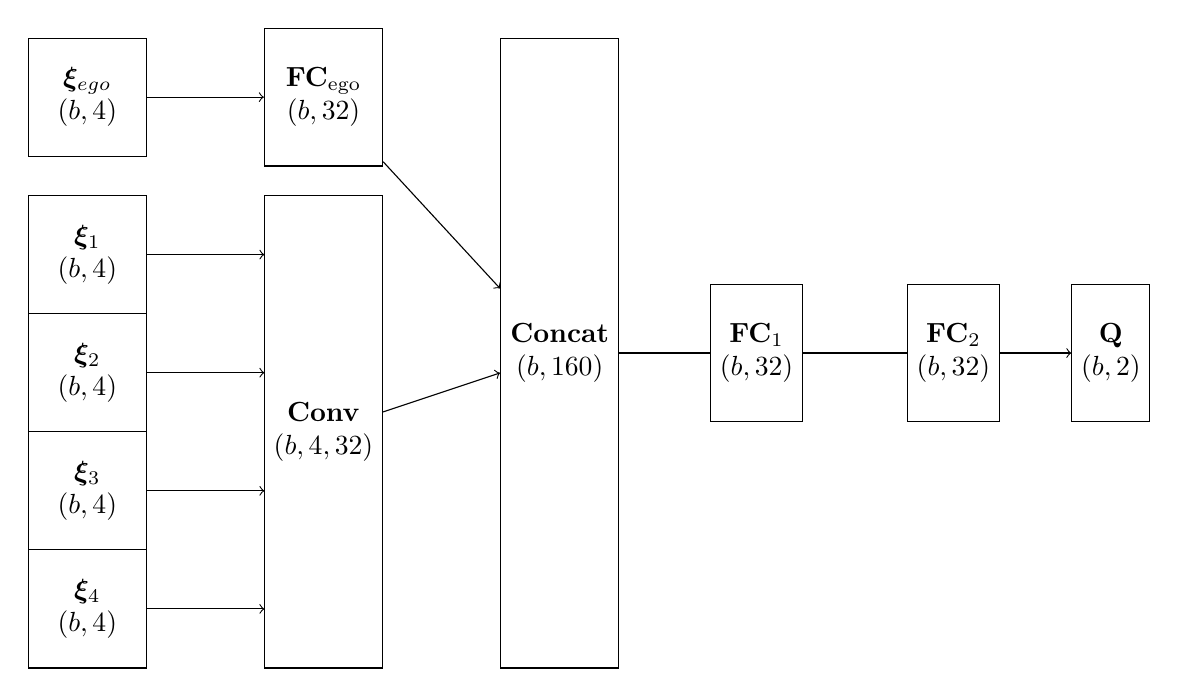
\begin{tikzpicture}
	
	\def\distlayers{3}

	\def\x{0}
	\def\y{0}
	\node [draw, rectangle,minimum width=1.5cm, minimum height=1.5cm, align=center] at (\x,\y) (input_ego){$\bm \xi_{ego}$ \\ $(b,4)$};
	\node [draw, rectangle,minimum width=1.5cm, minimum height=1.75cm, align=center] at (\x+\distlayers,\y) (fc_ego){\textbf{FC}$_{\mathrm{ego}}$ \\ $(b,32)$};
	\draw [->] (input_ego) -- (fc_ego);
	% taget input layers
	\def\x{0}
	\def\y{-2}

	% \foreach \i [evaluate=\i as \y using int((\i-1) * 2)] in {1,...,4}
	\foreach \i in {1,...,4}
	{
		\node [draw, rectangle,minimum width=1.5cm, minimum height=1.5cm, align=center] at (\x,\y) (input\i){$\bm \xi_{\i}$ \\ $(b,4)$};
		\node [coordinate] at (\x+2.25, \y) (first_layer\i){};
		\draw [->] (input\i) -- (first_layer\i);
		\pgfmathparse{\y - 1.5}
		\xdef\y{\pgfmathresult}
	}
	
	% CNN
	\def\x{\distlayers}
	\def\y{-2}
	\node [draw, rectangle,minimum width=1.5cm, minimum height=6cm, align=center] at (\x, \y-2.25) (cnn){\textbf{Conv} \\ $(b,4, 32)$};

	% concat layer
	\node [draw, rectangle,minimum width=1.5cm, minimum height=8cm, align=center] at (\x +\distlayers, \y-1.25) (concat){\textbf{Concat} \\ $(b,160)$};
	\draw [->] (cnn) -- (concat);
	\draw [->] (fc_ego) -- (concat);
	
	% FC layers to output 
	\foreach \layer [count=\i] in {concat,fc1}
	{
		\node [draw, rectangle, minimum width=1.0cm, minimum height=1.75cm, align=center, right of=\layer, node distance=2.5 cm] (fc\i){\textbf{FC}$_{\mathrm{\i}}$ \\ $(b,32)$};
	}

	\node [draw, rectangle, minimum width=0.75cm, minimum height=1.75cm, align=center, right of=fc2, node distance=2 cm] (Q){\textbf{Q} \\ $(b,2)$};
	\draw [->] (concat) -- (fc1) -- (fc2) -- (Q);
	
	\end{tikzpicture}
	\endpgfgraphicnamed
	
	\tikzstyle{arrow} = [thick,->,>=stealth, line width=1pt]
	\tikzstyle{darrow} = [thick,<->,>=stealth, line width=1pt]

	\beginpgfgraphicnamed{figures-old_network}
	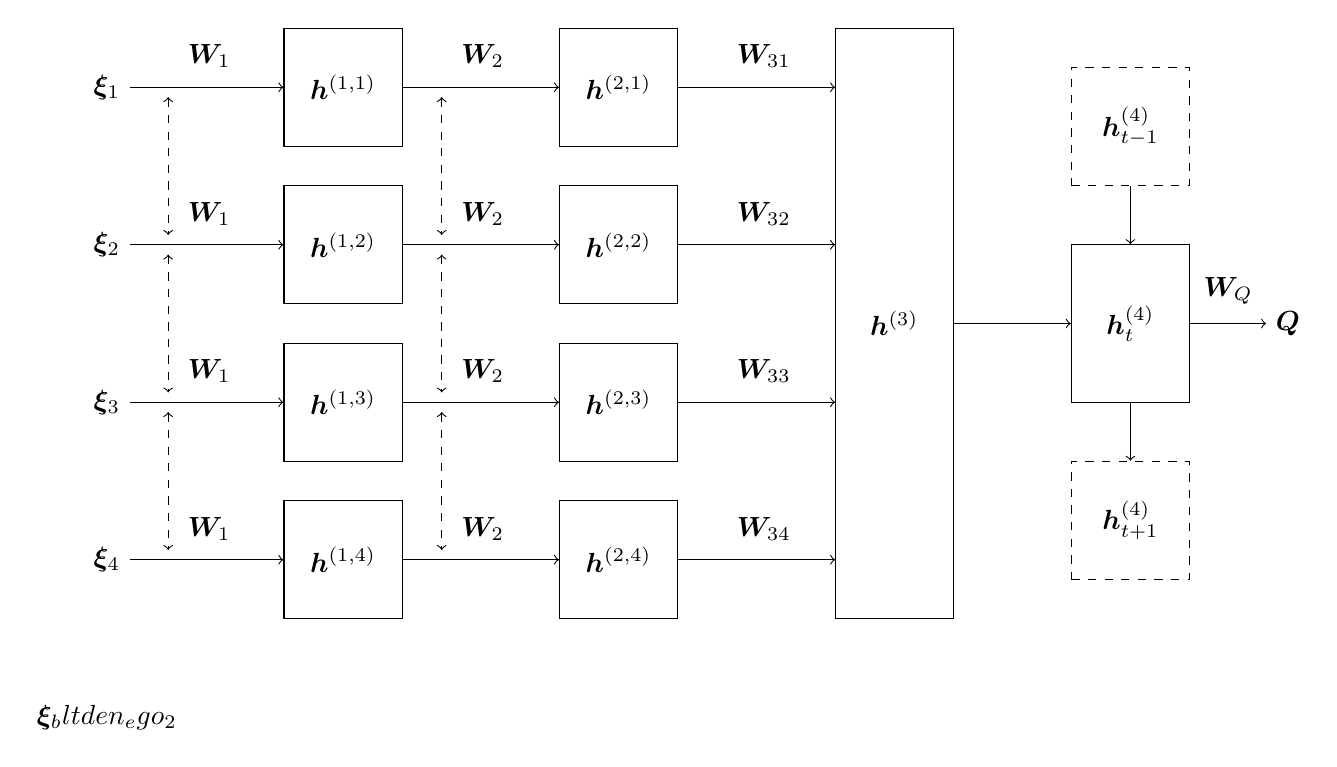
\begin{tikzpicture}
	
	\node [] at (0, 0) (input1){$\bm\xi_{1}$};
	\node [draw, rectangle,minimum width=1.5cm, minimum height=1.5cm] at (3, 0) (hidden1_1){$\bm h^{(1,1)}$};
	\node [draw, rectangle,minimum width=1.5cm, minimum height=1.5cm] at (6.5, 0) (hidden1_2){$\bm h^{(2,1)}$};
	\node [coordinate] at (9.25, 0) (hidden_combined1){};
	
	\node [] at (0, -2) (input2){$\bm\xi_{2}$};
	\node [draw, rectangle,minimum width=1.5cm, minimum height=1.5cm] at (3, -2) (hidden2_1){$\bm h^{(1,2)}$};
	\node [draw, rectangle,minimum width=1.5cm, minimum height=1.5cm] at (6.5, -2) (hidden2_2){$\bm h^{(2,2)}$};
	\node [coordinate] at (9.25, -2) (hidden_combined2){};
	
	\node [] at (0, -4) (input3){$\bm\xi_{3}$};
	\node [draw, rectangle,minimum width=1.5cm, minimum height=1.5cm] at (3, -4) (hidden3_1){$\bm h^{(1,3)}$};
	\node [draw, rectangle,minimum width=1.5cm, minimum height=1.5cm] at (6.5, -4) (hidden3_2){$\bm h^{(2,3)}$};
	\node [coordinate] at (9.25, -4) (hidden_combined3){};
	
	\node [] at (0, -6) (input4){$\bm\xi_{4}$};
	\node [draw, rectangle,minimum width=1.5cm, minimum height=1.5cm] at (3, -6) (hidden4_1){$\bm h^{(1,4)}$};
	\node [draw, rectangle,minimum width=1.5cm, minimum height=1.5cm] at (6.5, -6) (hidden4_2){$\bm h^{(2,4)}$};
	\node [coordinate] at (9.25, -6) (hidden_combined4){};
	
	\foreach \x in {1,...,4}{
		\draw [->] (input\x) -- node [near start,label=above right:$\bm W_1$] (w\x_1) {} (hidden\x_1);
		\draw [->] (hidden\x_1) -- node [near start,label=above right:$\bm W_2$] (w\x_2) {} (hidden\x_2);
		\draw [->] (hidden\x_2) -- node [near start,label=above right:$\bm W_{3\x}$] (w\x_3) {} (hidden_combined\x);
	}
	
	\node [] at (0, -8) (input){$\bm \xi_bltden_ego_2$};
	
	\draw [<->, dashed] (w1_1) -- (w2_1);
	\draw [<->, dashed] (w1_2) -- (w2_2);
	\draw [<->, dashed] (w2_1) -- (w3_1);
	\draw [<->, dashed] (w2_2) -- (w3_2);
	\draw [<->, dashed] (w3_1) -- (w4_1);
	\draw [<->, dashed] (w3_2) -- (w4_2);
	
	\node [draw, rectangle,minimum width=1.5cm, minimum height=7.5cm] at (10, -3) (hidden_combined){$\bm h^{(3)}$};
	
	\node [draw, dashed, rectangle,minimum width=1.5cm, minimum height=1.5cm] at (13, -0.5) (lstm_t_minus1){$\bm h^{(4)}_{t-1}$};
	\node [draw, rectangle,minimum width=1.5cm, minimum height=2cm] at (13, -3) (lstm_t){$\bm h^{(4)}_{t}$};
	\node [draw, dashed, rectangle,minimum width=1.5cm, minimum height=1.5cm] at (13, -5.5) (lstm_t_plus1){$\bm h^{(4)}_{t+1}$};
	
	\draw [->] (hidden_combined) -- (lstm_t);
	
	\draw [->] (lstm_t_minus1) -- (lstm_t);
	\draw [->] (lstm_t) -- (lstm_t_plus1);
	
	\node [] at (15, -3) (output){$\bm{Q}$};
	
	\draw [->] (lstm_t) -- node [midway,label=above:$\bm W_{Q}$] (w_o) {} (output);
	
	\end{tikzpicture}
	\endpgfgraphicnamed

	\tikzstyle{arrow} = [thick,->,>=stealth, line width=1pt]
	\tikzstyle{darrow} = [thick,<->,>=stealth, line width=1pt]
	
	\beginpgfgraphicnamed{figures-mpc_architecture}%
	\begin{tikzpicture}
	
	% Dashed rectangle
	\node[draw,thick,dashed,gray,rectangle,rounded corners =0.05cm,minimum width=6cm,minimum height = 3.5cm]  at (0.25,-0.35) {} ;
	
	% Box for A
	\node[draw,thick,rectangle,rounded corners =0.05cm,fill=gray!10,minimum width=2cm,minimum height = 0.5cm] (A) at (2.5,2) {Environment};
	
	% Box for B
	\node[draw,thick,rectangle,rounded corners =0.05cm,fill=gray!10,minimum width=2cm,minimum height = 2cm] (B) at (-1.5,0) {};
	% Separate text a bit under SQP
	\node at (-1.5,-0.25) {Policy};
	
	% Box for C
	\node[draw,thick,rectangle,rounded corners =0.05cm,fill=gray!10,minimum width=2cm,minimum height = 2cm] (C) at (2,0) {Controller};
	
	%  Box for D
	\node[draw,rectangle,thick,rounded corners =0.05cm,fill=gray!10,minimum width=2cm,minimum height = 2cm] (D) at (6.5,0) {Vehicle};
	
	% Arrow from B to C
	\draw[arrow,thick] (B) --(C) node [midway,above] {Action};
	
	% Arrow from C to D
	\draw[arrow,thick] (C) --(D) node [midway,above] {Acceleration};
	
	% Arrow from top of D up and then to A
	\draw[arrow,thick] (D.north) |- (A.east);
	
	%  Arrow from left of A to left  to down
	\draw[arrow,thick] (A.west) --+(-2.5,0) node[midway,xshift=1cm,above left]
	{Observation} -| (B.north);
	
	% Draw inside box
	
	\node[draw,thick,fill=gray!10,rectangle,rounded corners=0.05cm,align=center,font=\footnotesize] (reward) at (0.25,-1.5) {Immediate \\ Reward};

	\draw[arrow, thick] (2,-1) to [out=-100, in=2] (reward);
	% Draw from inside box to B
	\draw[arrow,thick] (reward) to [out=178, in=-70] (-1.5, -1);
	
	% Draw box inside of B
	\node[draw,thick,dashed, fill=gray!10,rectangle,rounded corners =0.05cm,align=center,font=\footnotesize]  (inside) at (-1.5,0.5) {State \\ Reward};
	
	\end{tikzpicture}
	\endpgfgraphicnamed
	
	\tikzstyle{arrow} = [thick,->,>=stealth, line width=1pt]
	\tikzstyle{darrow} = [thick,<->,>=stealth, line width=1pt]

	\beginpgfgraphicnamed{figures-system_architecture}%
	\begin{tikzpicture}[
		node distance=8mm and 30mm,
		node font= \Large,
		box/.style = {draw, thick, rectangle, rounded corners=0.1cm, fill=gray!10, minimum width=3.5cm, minimum height=2cm, align=center},
		sx+/.style = {xshift = 2mm},
		sx+/.style = {xshift = 2mm}
		]

		% \node[draw,thick,rectangle,rounded corners =0.05cm,fill=gray!10,minimum width=2cm,minimum height = 2cm] (SF) at (2,0) {Sensor Fusion};
		
		% \draw[arrow,thick] (0,0) --(SF) node [midway,above] {Sensors: Lidar, Radar, Camera, Sonar};

		% \node[draw,thick,rectangle,rounded corners =0.05cm,fill=gray!10,minimum width=2cm,minimum height = 2cm, shift={(2,0,0)}] (SF) at (2,0) {Sensor \\ Fusion};
		
		\node (start) at (0,0) {};
		\node (SF) [box, right=of start.east] {Sensor \\ Fusion};
		\node (PS) [box, right=of SF.east] {Precautionary \\ Safety};
		\node (DM) [box, right=of PS.east] {Decision \\ Maker};
		\node (Con) [box, right=of DM.east] {Controller};
		\node (CA) [box, below=of Con] {Collision \\ Avoidance};
		\node (Act) [box, right=of Con.east] {Actuator};
		\node (end) [right=of Act] {};


		\draw[arrow,thick,align=left] (start) --+(SF) node [midway,above] {Lidar\\Camera\\etc.};
		\draw[arrow,thick,align=left] (SF) --+(PS) node [midway,above] {Position\\Velocity\\etc.};
		\draw[arrow,thick,align=left] (PS) --+(DM) node [midway,above] {Safe\\Actions};
		\draw[arrow,thick,align=left] (DM) --+(Con) node [midway,above] {Action\\Reference};
		\draw[arrow,thick,align=left] (DM) -| ($(DM.east) + (1.5,0mm)$) |- (CA) node [midway,above] {};
		\draw[arrow,thick,align=left] (CA) -| ($(CA.east) + (1.5,0mm)$) |- (Act) node [midway,above] {};
		\draw[arrow,thick,align=left] (Con) --+(Act) node [midway,above] {Acceleration\\Request};
		\draw[arrow,thick,align=left] (Act) --+(end) node [midway,above] {};


	% --> Sensor Fusion --> Precautionary Safety --> |Decision Maker --> Controller |--> Actuator -->
	% 																->Collision Avoidance |

	\end{tikzpicture}
	\endpgfgraphicnamed

	\tikzstyle{arrow} = [thick,->,>=stealth, line width=1pt]
	\tikzstyle{darrow} = [thick,<->,>=stealth, line width=1pt]
	
	\beginpgfgraphicnamed{figures-algorithms}%
	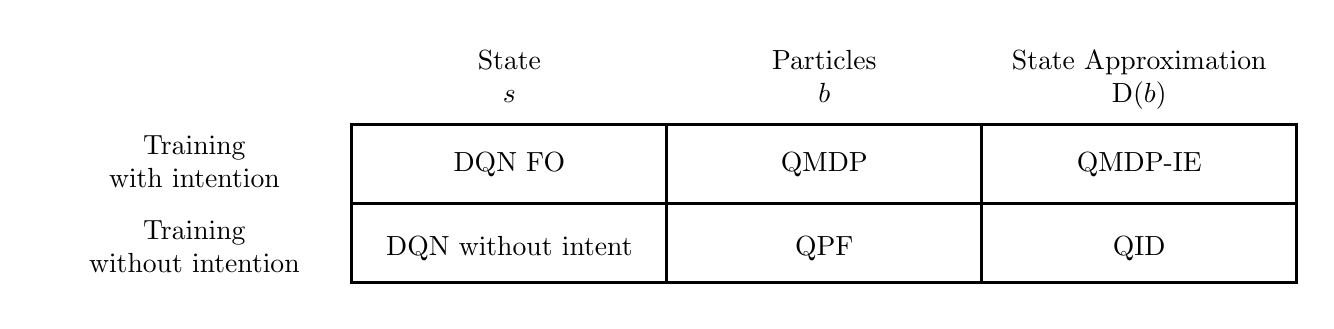
\begin{tikzpicture}
		\matrix (algo-text) [matrix of nodes,nodes={minimum width=4cm,minimum height=1cm}]
		{    & \makecell{State \\ $s$} & \makecell{Particles \\ $b$} & \makecell{State Approximation \\  $\text{D}(b)$ } & \\
			\makecell{Training \\ with intention} & DQN FO & QMDP & QMDP-IE \\
			\makecell{Training \\ without intention} & DQN without intent & QPF & QID \\
		};
		\def\y{-0.5}
		\draw[draw=black,line width=1pt] (-4,\y) rectangle ++(4,1);
		\draw[draw=black,line width=1pt] (-0,\y) rectangle ++(4,1);
		\draw[draw=black,line width=1pt] (4,\y) rectangle ++(4,1);
		\draw[draw=black,line width=1pt] (-4,\y-1) rectangle ++(4,1);
		\draw[draw=black,line width=1pt] (-0,\y-1) rectangle ++(4,1);
		\draw[draw=black,line width=1pt] (4,\y-1) rectangle ++(4,1);

		% \draw[draw=black] (-8,0) rectangle ++(4,1);
		% \node[draw,thick,rectangle,align=center,font=\footnotesize] (fo) at (-8,0) {FO \\ Reward};
		% \node[draw,thick,rectangle,align=center,font=\footnotesize, right of=fo] (qmdp) {QMDP \\ Reward};
		% \matrix (algo-frames) [matrix of nodes,nodes={minimum width=4cm,minimum height=1cm,draw,very thin}]
		% {   
		% 	" &  &  &  \\
		% 	"  &  &  &  \\
		% };

		% \draw[thick,violet] (magic-2-1.east) to[out=180,in=270,looseness=0.5] (magic-2-1.north) to[out=270,in=0,looseness=0.5] (magic-2-1.west) to[out=0,in=90,looseness=0.5] (magic-2-1.south) to[out=90,in=180,looseness=0.5] (magic-2-1.east);
		% \draw[rounded corners=2pt,densely dashed,green!50!gray] ($(magic-1-2.center)+(-0.15,-0.25)$) rectangle ($(magic-1-3.center)+(0.15,0.25)$);
	
	\end{tikzpicture}
	\endpgfgraphicnamed

	\tikzstyle{arrow} = [thick,->,>=stealth, line width=1pt]
	\tikzstyle{darrow} = [thick,<->,>=stealth, line width=1pt]

	\beginpgfgraphicnamed{figures-1-4cars}%
	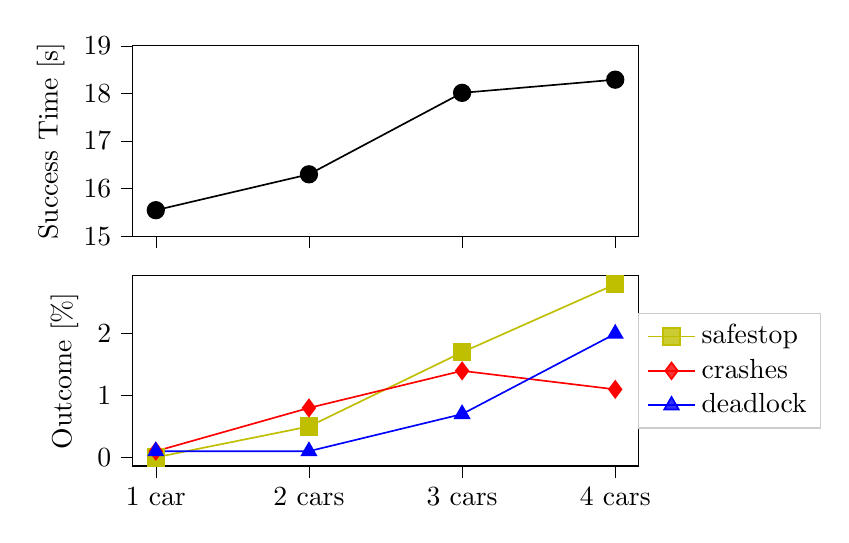
\begin{tikzpicture}

	\definecolor{darkgray176}{RGB}{176,176,176}
	\definecolor{goldenrod1911910}{RGB}{191,191,0}
	\definecolor{lightgray204}{RGB}{204,204,204}
	
	\begin{groupplot}[group style={group size=1 by 2, vertical sep = 0.5 cm},
		width = 8 cm,
    height = 4 cm]
	\nextgroupplot[
	scaled x ticks=manual:{}{\pgfmathparse{#1}},
	tick align=outside,
	tick pos=left,
	x grid style={darkgray176},
	xmin=-0.15, xmax=3.15,
	xtick style={color=black},
	xtick={0,1,2,3},
	xticklabels={1 car,2 cars,3 cars,4 cars},
	xticklabels={},
	y grid style={darkgray176},
	ylabel={Success Time [s]},
	ymin=15, ymax=19,
	ytick style={color=black}
	]
	\addplot [semithick, black, mark=*, mark size=3, mark options={solid}]
	table {%
	0 15.5470941883768
	1 16.3007099391481
	2 18.0119542619543
	3 18.288522848034
	};
	
	\nextgroupplot[
	legend cell align={left},
	legend style={
		fill opacity=0.8,
		draw opacity=1,
		text opacity=1,
		at={(1,0.5)},
		anchor=west,
		draw=lightgray204
	},
	tick align=outside,
	tick pos=left,
	x grid style={darkgray176},
	xmin=-0.15, xmax=3.15,
	xtick style={color=black},
	xtick={0,1,2,3},
	xtick={0,1,2,3},
	xtick={0,1,2,3},
	xtick={0,1,2,3},
	xticklabels={1 car,2 cars,3 cars,4 cars},
	xticklabels={1 car,2 cars,3 cars,4 cars},
	xticklabels={1 car,2 cars,3 cars,4 cars},
	xticklabels={1 car,2 cars,3 cars,4 cars},
	y grid style={darkgray176},
	ylabel={Outcome [\%]},
	ymin=-0.14, ymax=2.94,
	ytick style={color=black}
	]
	\addplot [semithick, goldenrod1911910, mark=square*, mark size=3, mark options={solid}]
	table {%
	0 0
	1 0.5
	2 1.7
	3 2.8
	};
	\addlegendentry{safestop}
	\addplot [semithick, red, mark=diamond*, mark size=3, mark options={solid}]
	table {%
	0 0.1
	1 0.8
	2 1.4
	3 1.1
	};
	\addlegendentry{crashes}
	\addplot [semithick, blue, mark=triangle*, mark size=3, mark options={solid}]
	table {%
	0 0.1
	1 0.1
	2 0.7
	3 2
	};
	\addlegendentry{deadlock}
	\end{groupplot}
	
	\end{tikzpicture}
	\endpgfgraphicnamed

	\tikzstyle{arrow} = [thick,->,>=stealth, line width=1pt]
	\tikzstyle{darrow} = [thick,<->,>=stealth, line width=1pt]

	\beginpgfgraphicnamed{figures-intention-t}%

	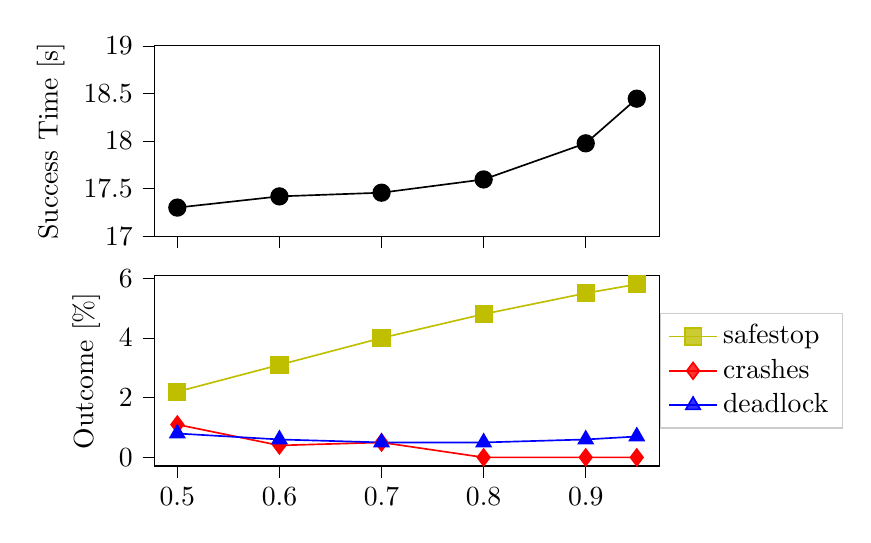
\begin{tikzpicture}

	\definecolor{darkgray176}{RGB}{176,176,176}
	\definecolor{goldenrod1911910}{RGB}{191,191,0}
	\definecolor{lightgray204}{RGB}{204,204,204}
	
	\begin{groupplot}[group style={group size=1 by 2, vertical sep = 0.5 cm},
		width = 8 cm,
        height = 4 cm]
	\nextgroupplot[
	scaled x ticks=manual:{}{\pgfmathparse{#1}},
	tick align=outside,
	tick pos=left,
	x grid style={darkgray176},
	xmin=0.4775, xmax=0.9725,
	xtick style={color=black},
	xticklabels={},
	y grid style={darkgray176},
	ylabel={Success Time [s]},
	ymin=17, ymax=19,
	ytick style={color=black}
	]
	\addplot [semithick, black, mark=*, mark size=3, mark options={solid}]
	table {%
	0.5 17.3008342022941
	0.6 17.4186652763295
	0.7 17.4573684210526
	0.8 17.5966209081309
	0.9 17.9760383386581
	0.95 18.4449197860963
	};
	
	\nextgroupplot[
	legend cell align={left},
	legend style={
		fill opacity=0.8,
		draw opacity=1,
		text opacity=1,
		at={(1,0.5)},
		anchor=west,
		draw=lightgray204
	},
	tick align=outside,
	tick pos=left,
	x grid style={darkgray176},
	xmin=0.4775, xmax=0.9725,
	xtick style={color=black},
	y grid style={darkgray176},
	ylabel={Outcome [\%]},
	ymin=-0.29, ymax=6.09,
	ytick style={color=black}
	]
	\addplot [semithick, goldenrod1911910, mark=square*, mark size=3, mark options={solid}]
	table {%
	0.5 2.2
	0.6 3.1
	0.7 4
	0.8 4.8
	0.9 5.5
	0.95 5.8
	};
	\addlegendentry{safestop}
	\addplot [semithick, red, mark=diamond*, mark size=3, mark options={solid}]
	table {%
	0.5 1.1
	0.6 0.4
	0.7 0.5
	0.8 0
	0.9 0
	0.95 0
	};
	\addlegendentry{crashes}
	\addplot [semithick, blue, mark=triangle*, mark size=3, mark options={solid}]
	table {%
	0.5 0.8
	0.6 0.6
	0.7 0.5
	0.8 0.5
	0.9 0.6
	0.95 0.7
	};
	\addlegendentry{deadlock}
	\end{groupplot}
	\end{tikzpicture}
	\endpgfgraphicnamed


	\tikzstyle{arrow} = [thick,->,>=stealth, line width=1pt]
	\tikzstyle{darrow} = [thick,<->,>=stealth, line width=1pt]

	
\newcommand{\diagramgraph}[3]{% #1=Image, #2=y-axis, #3=x-axis
	\begin{sideways}
		\parbox{\heightof{#1}}{%
			\raggedright \centering \scalebox{0.9}[0.9]{\bf{\sffamily\footnotesize#2}}}%
	\end{sideways}%
	\mbox{#1\hspace{.5\baselineskip}}%
	\\
	\parbox{\widthof{#1}}{%
		\raggedright \centering \hspace{0.7cm} \scalebox{0.9}[0.9]{\bf{\sffamily\footnotesize#3}}}
}

\newcommand{\graphwithlegend}[6]{% #1=image, #2=toplegend, #3=color #4bottomlegend #5color #6 location
	\begin{tikzpicture}[every node/.style={inner sep=.05cm,outer sep=0cm}]
	\node[anchor=south east] at (0,0) {#1};
	\node[anchor=south east,draw=gray, fill=white!20] at (#6) {
		\sffamily \footnotesize \scalebox{.4}[0.4]{
			\begin{tabular}{@{}rl@{}}
			\textcolor[rgb]{#3}{$\blacksquare$} & #2 \\
			\textcolor[rgb]{#5}{$\blacksquare$} & #4 \\
			\end{tabular}
		}
	};
	\end{tikzpicture}
}

\newcommand{\resultgraphwithlegend}[5]{% #1=image_file, #2=toplegend, #3=color #4bottomlegent #5color
	\begin{minipage}{0.35\textwidth}
		\diagramgraph{\graphwithlegend{\includegraphics[trim={0 0 -.5cm .0cm},clip,width=.95\textwidth]{#1}}{#2}{#3}{#4}{#5}{-.4, 0.6}}{success rate}{training episode}
	\end{minipage}
	\vspace{-0.5cm}
}

\newcommand{\crashgraphwithlegend}[5]{% #1=image_file, #2=toplegend, #3=color #4bottomlegent #5color
	\begin{minipage}{0.35\textwidth}
		\diagramgraph{\graphwithlegend{\includegraphics[trim={0 0 -.5cm .0cm},clip,width=.95\textwidth]{#1}}{#2}{#3}{#4}{#5}{-.4, 0.6}}{Crash Timeout Ratio}{training episode}
	\end{minipage}
	\vspace{-0.5cm}
}

% \beginpgfgraphicnamed{figures-successrate}
% \resultgraphwithlegend{successrate_single.png}{SM}{0.93,0.47,0.31}{MPC}{0.36,0.73,0.91}
% \endpgfgraphicnamed

% \beginpgfgraphicnamed{figures-crashratio}
% \crashgraphwithlegend{crashratio_single.png}{SM}{0.93,0.47,0.31}{MPC}{0.36,0.73,0.91}
% \endpgfgraphicnamed


%\begin{minipage}{0.32\textwidth}
%	\diagramgraph{
\includegraphics[trim={0 0 -.5cm .7cm},clip,width=.95\textwidth]{ego_car_top_down.png}}{success rate}{training episode}
%\end{minipage}

%\beginpgfgraphicnamed{figures-recurrent}
%\resultgraphwithlegend{results_recurrent.png}{DRQN}{0.74,0.25,0.14}{DQN}{0.26,0.59,0.53}
%\endpgfgraphicnamed


\end{document}